%%%%%%%%%%%%%%%%%%%%%%%%%%%%%%%%%%%%%%%%%%%%%%%%%%%%%%%%%%%%%%%%%%%%%%%%%%%%%%%%
%%%%%%%%%%%%%%%%%%%%%%%%%%%%%%%%%%%%%%%%%%%%%%%%%%%%%%%%%%%%%%%%%%%%%%%%%%%%%%%%
%%                                                                            %%
%% thesistemplate.tex version 3.20 (2018/08/31)                               %%
%% The LaTeX template file to be used with the aaltothesis.sty (version 3.20) %%
%% style file.                                                                %%
%% This package requires pdfx.sty v. 1.5.84 (2017/05/18) or newer.            %%
%%                                                                            %%
%% This is licensed under the terms of the MIT license below.                 %%
%%                                                                            %%
%% Written by Luis R.J. Costa.                                                %%
%% Currently developed at the Learning Services of Aalto University School of %%
%% Electrical Engineering by Luis R.J. Costa since May 2017.                  %%
%%                                                                            %%
%% Copyright 2017-2018, by Luis R.J. Costa, luis.costa@aalto.fi,              %%
%% Copyright 2017-2018 Swedish translations in aaltothesis.cls by Elisabeth   %%
%% Nyberg, elisabeth.nyberg@aalto.fi and Henrik Wallén,                       %%
%% henrik.wallen@aalto.fi.                                                    %%
%% Copyright 2017-2018 Finnish documentation in the template opinnatepohja.tex%%
%% by Perttu Puska, perttu.puska@aalto.fi, and Luis R.J. Costa.               %%
%% Copyright 2018 English template thesistemplate.tex by Luis R.J. Costa.     %%
%% Copyright 2018 Swedish template kandidatarbetsbotten.tex by Henrik Wallen. %%
%%                                                                            %%
%% Permission is hereby granted, free of charge, to any person obtaining a    %%
%% copy of this software and associated documentation files (the "Software"), %%
%% to deal in the Software without restriction, including without limitation  %%
%% the rights to use, copy, modify, merge, publish, distribute, sublicense,   %%
%% and/or sell copies of the Software, and to permit persons to whom the      %%
%% Software is furnished to do so, subject to the following conditions:       %%
%% The above copyright notice and this permission notice shall be included in %%
%% all copies or substantial portions of the Software.                        %%
%% THE SOFTWARE IS PROVIDED "AS IS", WITHOUT WARRANTY OF ANY KIND, EXPRESS OR %%
%% IMPLIED, INCLUDING BUT NOT LIMITED TO THE WARRANTIES OF MERCHANTABILITY,   %%
%% FITNESS FOR A PARTICULAR PURPOSE AND NONINFRINGEMENT. IN NO EVENT SHALL    %%
%% THE AUTHORS OR COPYRIGHT HOLDERS BE LIABLE FOR ANY CLAIM, DAMAGES OR OTHER %%
%% LIABILITY, WHETHER IN AN ACTION OF CONTRACT, TORT OR OTHERWISE, ARISING    %%
%% FROM, OUT OF OR IN CONNECTION WITH THE SOFTWARE OR THE USE OR OTHER        %%
%% DEALINGS IN THE SOFTWARE.                                                  %%
%%                                                                            %%
%%                                                                            %%
%%%%%%%%%%%%%%%%%%%%%%%%%%%%%%%%%%%%%%%%%%%%%%%%%%%%%%%%%%%%%%%%%%%%%%%%%%%%%%%%
%%                                                                            %%
%%                                                                            %%
%% An example for writting your thesis using LaTeX                            %%
%% Original version and development work by Luis Costa, changes to the text   %%
%% in the Finnish template by Perttu Puska.                                   %%
%% Support for Swedish added 15092014                                         %%
%% PDF/A-b support added on 15092017                                          %%
%% PDF/A-2 support added on 24042018                                          %%
%%                                                                            %%
%% This example consists of the files                                         %%
%%         thesistemplate.tex (version 3.20) (for text in English)            %%
%%         opinnaytepohja.tex (version 3.20) (for text in Finnish)            %%
%%         kandidatarbetsbotten.tex (version 1.00) (for text in Swedish)      %%
%%         aaltothesis.cls (versio 3.20)                                      %%
%%         kuva1.eps (graphics file)                                          %%
%%         kuva2.eps (graphics file)                                          %%
%%         kuva1.jpg (graphics file)                                          %%
%%         kuva2.jpg (graphics file)                                          %%
%%         kuva1.png (graphics file)                                          %%
%%         kuva2.png (graphics file)                                          %%
%%         kuva1.pdf (graphics file)                                          %%
%%         kuva2.pdf (graphics file)                                          %%
%%                                                                            %%
%%                                                                            %%
%% Typeset in Linux either with                                               %%
%% pdflatex: (recommended method)                                             %%
%%             $ pdflatex thesistemplate                                      %%
%%             $ pdflatex thesistemplate                                      %%
%%                                                                            %%
%%   The result is the file thesistemplate.pdf that is PDF/A compliant, if    %%
%%   you have chosen the proper \documenclass options (see comments below)    %%
%%   and your included graphics files have no problems.
%%                                                                            %%
%% Or                                                                         %%
%% latex: (this method is not recommended)                                    %%
%%             $ latex thesistemplate                                         %%
%%             $ latex thesistemplate                                         %%
%%                                                                            %%
%%   The result is the file thesistemplate.dvi, which is converted to ps      %%
%%   format as follows:                                                       %%
%%                                                                            %%
%%             $ dvips thesistemplate -o                                      %%
%%                                                                            %%
%%   and then to pdf as follows:                                              %%
%%                                                                            %%
%%             $ ps2pdf thesistemplate.ps                                     %%
%%                                                                            %%
%%   This pdf file is not PDF/A compliant. You must must make it so using,    %%
%%   e.g., Acrobat Pro or PDF-XChange.                                        %%
%%                                                                            %%
%%                                                                            %%
%% Explanatory comments in this example begin with the characters %%, and     %%
%% changes that the user can make with the character %                        %%
%%                                                                            %%
%%%%%%%%%%%%%%%%%%%%%%%%%%%%%%%%%%%%%%%%%%%%%%%%%%%%%%%%%%%%%%%%%%%%%%%%%%%%%%%%
%%%%%%%%%%%%%%%%%%%%%%%%%%%%%%%%%%%%%%%%%%%%%%%%%%%%%%%%%%%%%%%%%%%%%%%%%%%%%%%%

%% USE one of these:
%% * the first when using pdflatex, which directly typesets your document in the
%%   chosen pdf/a format and you want to publish your thesis online,

%% * the second when you want to print your thesis to bind it, or
%% * the third when producing a ps file and a pdf/a from it.
%%
\documentclass[english, 12pt, a4paper, sci, utf8, online]{aaltothesis}
%\documentclass[english, 12pt, a4paper, elec, utf8, a-1b]{aaltothesis}
%\documentclass[english, 12pt, a4paper, elec, dvips, online]{aaltothesis}

%% Use the following options in the \documentclass macro above:
%% your school: arts, biz, chem, elec, eng, sci
%% the character encoding scheme used by your editor: utf8, latin1
%% thesis language: english, finnish, swedish
%% make an archiveable PDF/A-1b or PDF/A-2b compliant file: a-1b, a-2b
%%                    (with pdflatex, a normal pdf containing metadata is
%%                     produced without the a-*b option)
%% typeset in symmetric layout and blue hypertext for online publication: online
%%            (no option is the default, resulting in a wide margin on the
%%             binding side of the page and black hypertext)
%% two-sided printing: twoside (default is one-sided printing)
%%

%% Use one of these if you write in Finnish (see the Finnish template
%% opinnaytepohja.tex)
%\documentclass[finnish, 12pt, a4paper, elec, utf8, a-1b, online]{aaltothesis}
%\documentclass[finnish, 12pt, a4paper, elec, utf8, a-1b]{aaltothesis}
%\documentclass[finnish, 12pt, a4paper, elec, dvips, online]{aaltothesis}

\usepackage{graphicx}

%% Math fonts, symbols, and formatting; these are usually needed
\usepackage{amsfonts,amssymb,amsbsy,amsmath}

%% Change the school field to specify your school if the automatically set name
%% is wrong
% \university{aalto-yliopisto}
% \school{Sähkötekniikan korkeakoulu}

%% Edit to conform to your degree programme
%%
\degreeprogram{Computer, Communication and Information Sciences}
%%

%% Your major
%%
\major{Computer Science}
%%

%% Major subject code
%%
\code{SCI3042}
%%

%% Choose one of the three below
%%
%\univdegree{BSc}
\univdegree{MSc}
%\univdegree{Lic}
%%

%% Your name (self explanatory...)
%%
\thesisauthor{Nikos Heikkilä}
%%

%% Your thesis title comes here and possibly again together with the Finnish or
%% Swedish abstract. Do not hyphenate the title, and avoid writing too long a
%% title. Should LaTeX typeset a long title unsatisfactorily, you mght have to
%% force a linebreak using the \\ control characters.
%% In this case...
%% Remember, the title should not be hyphenated!
%% A possible "and" in the title should not be the last word in the line, it
%% begins the next line.
%% Specify the title again without the linebreak characters in the optional
%% argument in box brackets. This is done because the title is part of the
%% metadata in the pdf/a file, and the metadata cannot contain linebreaks.
%%
\thesistitle{Title of the thesis}
%\thesistitle[Title of the thesis]{Title of\\ the thesis}
%%

%%
\place{Espoo}
%%

%% The date for the bachelor's thesis is the day it is presented
%%
\date{31.8.2018} % TODO change when date known
%%

%% Thesis supervisor
%% Note the "\" character in the title after the period and before the space
%% and the following character string.
%% This is because the period is not the end of a sentence after which a
%% slightly longer space follows, but what is desired is a regular interword
%% space.
%%
\supervisor{Prof.\ Jukka Suomela}
%%

%% Advisor(s)---two at the most---of the thesis. Check with your supervisor how
%% many official advisors you can have.
%%
\advisor{Dr.\ Chetan Gupta}
%\advisor{MSc Sarah Scientist}
%%

%% Aaltologo: syntax:
%% \uselogo{aaltoRed|aaltoBlue|aaltoYellow|aaltoGray|aaltoGrayScale}{?|!|''}
%% The logo language is set to be the same as the thesis language.
%%
\uselogo{aaltoRed}{''}
%%

%% The English abstract:
%% All the details (name, title, etc.) on the abstract page appear as specified
%% above.
%% Thesis keywords:
%% Note! The keywords are separated using the \spc macro
%%
\keywords{For keywords choose\spc concepts that are\spc central to your\spc thesis}
%%

%% The abstract text. This text is included in the metadata of the pdf file as well
%% as the abstract page.
%%
\thesisabstract{
Your abstract in English. Keep the abstract short. The abstract explains your
research topic, the methods you have used, and the results you obtained. In the
PDF/A format of this thesis, in addition to the abstract page, the abstract text is
written into the pdf file's metadata. Write here the text that goes into the
metadata. The metadata cannot contain special characters, linebreak or paragraph
break characters, so these must not be used here. If your abstract does not contain
special characters and it does not require paragraphs, you may take advantage of
the abstracttext macro (see the comment below). Otherwise, the metadata abstract
text must be identical to the text on the abstract page.
}

%% Copyright text. Copyright of a work is with the creator/author of the work
%% regardless of whether the copyright mark is explicitly in the work or not.
%% You may, if you wish, publish your work under a Creative Commons license (see
%% creaticecommons.org), in which case the license text must be visible in the
%% work. Write here the copyright text you want. It is written into the metadata
%% of the pdf file as well.
%% Syntax:
%% \copyrigthtext{metadata text}{text visible on the page}
%%
%% In the macro below, the text written in the metadata must have a \noexpand
%% macro before the \copyright special character, and macros (\copyright and
%% \year here) must be separated by the \ character (space chacter) from the
%% text that follows. The macros in the argument of the \copyrighttext macro
%% automatically insert the year and the author's name. (Note! \ThesisAuthor is
%% an internal macro of the aaltothesis.cls class file).
%% Of course, the same text could have simply been written as
%% \copyrighttext{Copyright \noexpand\copyright\ 2018 Eddie Engineer}
%% {Copyright \copyright{} 2018 Eddie Engineer}
%%
\copyrighttext{Copyright \noexpand\copyright\ \number\year\ \ThesisAuthor}
{Copyright \copyright{} \number\year{} \ThesisAuthor}

%% You can prevent LaTeX from writing into the xmpdata file (it contains all the
%% metadata to be written into the pdf file) by setting the writexmpdata switch
%% to 'false'. This allows you to write the metadata in the correct format
%% directly into the file thesistemplate.xmpdata.
%\setboolean{writexmpdatafile}{false}

% Bibliography
\usepackage[
    backend=bibtex, % TODO change backend
    style=numeric,
    sorting=ynt
]{biblatex}
\addbibresource{refs.bib}

% My extra plugins
\usepackage[textwidth=1in, textsize=footnotesize]{todonotes}
\usepackage[]{tikz}
\usetikzlibrary{positioning,chains,fit,shapes,calc,quotes,matrix}
\usetikzlibrary{arrows.meta,arrows}

\tikzset{main node/.style={circle,fill=blue!20,draw,minimum size=1cm,inner sep=0pt}}
%% All that is printed on paper starts here
%%
\usepackage{caption}
\usepackage{subcaption}

% Commands

% Definitions
\definecolor{myblue}{RGB}{122,152,255}
\definecolor{myorange}{RGB}{255,190,103}

%\DeclareMathOperator{\deg}{deg} % This was already declared

\begin{document}

%% Create the coverpage
%%
\makecoverpage

%% Typeset the copyright text.
%% If you wish, you may leave out the copyright text from the human-readable
%% page of the pdf file. This may seem like a attractive idea for the printed
%% document especially if "Copyright (c) yyyy Eddie Engineer" is the only text
%% on the page. However, the recommendation is to print this copyright text.
%%
\makecopyrightpage

%% Note that when writting your thesis in English, place the English abstract
%% first followed by the possible Finnish or Swedish abstract.

%!tex root = ../main.tex
%% Abstract text
%% All the details (name, title, etc.) on the abstract page appear as specified
%% above.
%%
\begin{abstractpage}[english]
Your abstract in English.
\end{abstractpage}


%% The text in the \thesisabstract macro is stored in the macro \abstractext, so
%% you can use the text metadata abstract directly as follows:
%%
%\begin{abstractpage}[english]
%	\abstracttext{}
%\end{abstractpage}

%% Force a new page so that the possible Finnish or Swedish abstract does not
%% begin on the same page
%%
\newpage

%!tex root = ../main.tex
%%
%% Abstract in Finnish.  Delete if you don't need it.
%%
% LTeX: enabled=false
\thesistitle{Ei-vakioaikaisten alarajojen etsiminen automaattisesti paikallisesti tarkastettaville merkitsemisongelmille LOCAL-mallissa}
\supervisor{Prof.\ Jukka Suomela}
\advisor{Dr.\ Chetan Gupta}
%\degreeprogram{Elektroniikka ja sähkötekniikka}
%\department{Elektroniikan ja nanotekniikan laitos}
%\major{Sopiva pääaine}
%% The keywords need not be separated by \spc now.
\keywords{Paikallisesti tarkastettavat merkitsemisongelmat, LOCAL-malli, porttinumerointimalli, hajautetut algoritmit, hajautettu laskenta}
%% Abstract text
\begin{abstractpage}[finnish]
Hajautettu laskenta on mitä tahansa laskentaa, johon osallistuu eri paikoissa sijaitsevia tietokoneita.
Sitä käytetään usein tilanteissa, joissa vaaditaan suurta laskentatehoa.
Hajautettua laskentaa hyödyntämällä voidaan ratkaista ison mittakaavan ongelmia, jotka olisivat epäkäytännöllisiä ratkaista keskitetyssä järjestelmässä.

Tässä työssä tutkitaan hajautetun laskennan teoreettista perustaa.
Olen kiinnostunut hajautetun laskennan porttinumerointimallista eli PN-mallista sekä LOCAL-mallista.
Näissä malleissa jokainen tietokoneverkon solmu suorittaa samaa algoritmia synkronisesti ja vaihtaa jokaisella viestintäkierroksella viestejä viereisten solmujen kanssa.
Näiden viestintäkierroksien välillä solmut voivat laskea äärettömän nopeasti.
Algoritmin nopeus on se kierrosten määrä, jonka jälkeen jokainen verkon solmu viimeistään lopettaa algoritmin suorittamisen.
Paikallisesti tarkastettavat merkitsemisongelmat (LCL-ongelmat) ovat verkko-ongelmaperhe, jossa jokainen yksittäinen solmu voi paikallisesti tarkistaa globaalin ratkaisun.

Hajautetun laskennan teoreettisen perustan tutkimuksissa on viime aikoina näkynyt kehityssuunta, jossa automatisoidaan LCL-ongelmien ylä- ja alarajojen löytäminen LOCAL-mallissa.
Tämän työ edistää kyseistä tutkimusalaa automatisoimalla LCL-ongelmien ei-vakioaikaisten alarajojen löytämisen LOCAL-mallissa.

Esittelen uuden algoritmin, joka tunnistaa, jos annetulle LCL-ongelmalle ei ole ratkaisua äärellisissä yhtenäisissä $(\Delta, \delta)$-säännöllisissä kaksijakoisissa moniverkoissa.
Tämän jälkeen näytän, että jos tällä ongelmalla ei ole ratkaisua kyseisessä verkkoperheessä, niin se ei ole ratkeava PN-mallissa.
Näytän myös, että jos annettu LCL-ongelma ei ole ratkeava PN-mallissa, niin sitä ei voi myöskään ratkaista vakioajassa LOCAL-mallissa.
Tästä seuraa, että esittelemäni algoritmi voi todistaa automaattisesti, että LCL-ongelma ei ole vakioajassa ratkeava.
Esittelen myös toteutuksen algoritmille, jotta voimme käytännössä löytää automaattisesti uusia alarajoja LCL-ongelmille LOCAL-mallissa.
Löydän tällä toteutuksella uusia alarajoja yhdeksälle LCL-ongelmalle ja tämän seurauksena yhdelle näistä ongelmista tunnetaan sen laskennallinen vaativuus tarkasti: ongelman ratkaiseminen vaatii $\Theta(\log^* n)$ viestintäkierrosta.
\end{abstractpage}
% LTeX: enabled=true


%% Force new page so that the Swedish abstract starts from a new page
\newpage

%!tex root = ../main.tex
%% Preface
%%
%% This section is optional. Remove it if you do not want a preface.
\mysection{Preface}
%\mysection{Esipuhe}
I would like to thank my supervisor Jukka Suomela for the idea for this thesis, for the opportunity to write this thesis, and to work as a research assistant in the research group.
I am grateful for the enormous amount of advice, comments, and support I have received from Jukka.
I would also like to thank my advisor Chetan Gupta for giving me invaluable advice and comments on my thesis.
Finally, I would like to thank my family and friends for supporting me during my academic journey.
This work was supported in part by the Academy of Finland, Grant 333837.
\vspace{5cm}

Helsinki, 30.5.2022
%TODO Change the date and location
\vspace{5mm}
{\hfill Nikos Heikkilä \hspace{1cm}}


%% Force a new page after the preface
%%
\newpage


%% Table of contents.
%%
\thesistableofcontents


%!tex root = ../main.tex

\mysection{Symbols and abbreviations}
%TODO this section is a template that I'll use in case I want to have a separate page for these
\subsection*{Symbols}

\begin{tabular}{ll}
$c$              & description of this symbol\\
\end{tabular}

\subsection*{Operators}

\begin{tabular}{ll}
$\nabla \times \mathbf{A}$              & description of this operator\\
\end{tabular}

\subsection*{Abbreviations}

\begin{tabular}{ll}
PN              & port-numbering\\
LCL             & locally checkable labelling\\
\end{tabular}



%% \clearpage is similar to \newpage, but it also flushes the floats (figures
%% and tables).
%%
\cleardoublepage

%!tex root = ../main.tex

\section{Introduction}  \label{sec:introduction}

Large problems often require large computational capacity.
Distributed computing is often considered when high amounts of computation power are required.
It is used to solve large scale problems that would otherwise be impractical to solve in a centralized system.
Distributed computing is \emph{any kind} of computing that is performed on a spatially distributed system
\cite{DBLP:books/el/leeuwen90/LamportL90}.

In this thesis, we will be studying the theoretical foundations of distributed computing.
Our main focus is on locally checkable labelling (LCL) problems...
%The idea of distributed computing is to locally solve a part of a global solution by communicating with other

\todo{fix}


\subsection{Objectives}
In this thesis, we aim to implement a tool that can automatically find lower bounds for LCL problems.
\todo{fix}

\subsection{Thesis structure}
We structure the thesis so that one can read the sections in sequential order.
Section \ref{sec:background} gives a succinct theoretical background to the \todo[orange][]{topic of this work.}
After the theoretical background, we discuss our research question \todo[red][]{(TODO or questions?)} in more detail in Section \ref{sec:research_question}.
In Section \ref{sec:prior_work} we discuss the prior work related to this thesis.


First it explains ... %TODO Update these when background is done

Section \ref{sec:implementation}
\todo{fix}

%% Leave page number of the first page empty
%%
\thispagestyle{empty}

\clearpage
%!tex root = ../main.tex
%% Background
%%
\section{Background}
\todo{Could also be named as "Theoretical background"}
To understand the implementation chapter \ref{sec:solution}, in this section we introduce relevant terminology and concepts.

\todo{Add info about section \ref{sec:graphs}}

In the first section (\ref{sec:distributed_computing}) of this chapter, we discuss about the essential concepts in the theory of distributed computing.
The section aims to explain the meaning of distributed computing and gives an introduction to the main model of distributed computing, \emph{message passing model}, from which many of the researched models inherit from.

The second and third sections discuss about the Port number model and local model respectively.
These are widely used models in the field and they are strongly related to the research showed in this paper.

We are trying to find lower bound proofs for LCL-problems in this paper, therefore it is essential to include a section entirely for them.
The fourth section (\ref{sec:lcl_problems}) is dedicated to LCL-problems.

Finally, in the last section (\ref{sec:previous_research}), we talk about previous research in the field and research that are more related to this thesis.

\subsection{Graphs} \label{sec:graphs}
In the real world, there are many objects that are somehow related to each other.
Such things can often be visualized by a diagrams that consists of points, and lines that connect a pair of points.
A graph is a mathematical concept that abstracts the relations of these objects.
In the literature, the points are called vertices and lines are called edges.
\cite{DBLP:books/others/BondyM76}

Mathematically, graph can be defined as a tuple $$G = (V, E)$$ where $V$ is the set of vertices and $E$ is the set of edges.
%Each vertex $v \in V$
Each edge $e \in E$ can also be thought as a tuple $e=(v, w), v, w \in V$, where vertices $v$ and $w$ are the endpoints of the edge $e$.
For example, $G=(\{1, 2, 3\}, \{(1, 2),(1, 3),(2, 3),(3, 2)\})$, and visualized it looks like the graph on figure \ref{fig:graph1:a}.

When the order of the vertices in an edge matters, we call the graph as a \emph{directed graph} or with the shortened variation \emph{digraph}.
For digraphs, the following statement must hold:
\begin{equation} \label{eq:1}
\forall v, w \in V, v \neq w: (v, w) \neq (w, v)
\end{equation}
In that case, the first vertex $v$ points to the vertex $w$.
Usually the edge is visualized as an arrow pointing from $v$ to $w$.
One example of a directed graph is a flow graph, in which the edges represent flows from a vertex to another vertex, as seen in the figure \ref{fig:graph1:a}.

\begin{figure}[h]
  \subcaptionbox{A simple directed graph.\label{fig:graph1:a}}%
    [.3\linewidth] {
    \centering
    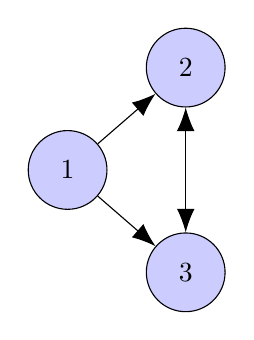
\begin{tikzpicture}[>={Latex[length=3mm]},auto, on grid, ]
      \node[main node] (1) {$1$};
      \node[main node] (2) [above right = 1.3cm and 1.5cm of 1] {$2$};
      \node[main node] (3) [below right = 1.3cm and 1.5cm of 1] {$3$};
      \draw[->] (1) edge[] node {} (2);
      \draw[->] (1) edge[] node {} (3);
      \draw[<->] (2) edge[] node {} (3);
    \end{tikzpicture}
  }
  \hfill
  \subcaptionbox{A simple undirected graph.\label{fig:graph1:b}}%
    [.3\linewidth] {
    \centering
    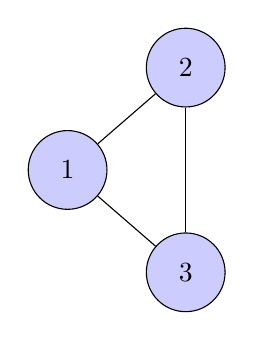
\begin{tikzpicture}[auto, on grid, ]
      \node[main node] (1) {$1$};
      \node[main node] (2) [above right = 1.3cm and 1.5cm of 1] {$2$};
      \node[main node] (3) [below right = 1.3cm and 1.5cm of 1] {$3$};
      \draw[-] (1) edge[] node {} (2);
      \draw[-] (1) edge[] node {} (3);
      \draw[-] (2) edge[] node {} (3);
    \end{tikzpicture}
  }
  \hfill
  \subcaptionbox{An undirected multigraph.\label{fig:graph1:c}}%
    [.3\linewidth] {
    \centering
    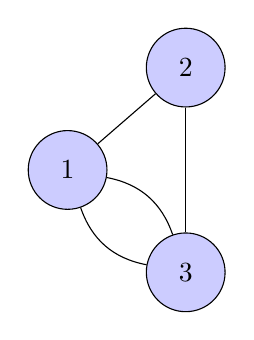
\begin{tikzpicture}[auto, on grid, ]
      \node[main node] (1) {$1$};
      \node[main node] (2) [above right = 1.3cm and 1.5cm of 1] {$2$};
      \node[main node] (3) [below right = 1.3cm and 1.5cm of 1] {$3$};
      \draw[-] (1) edge[] node {} (2);
      \draw[-] (1) edge[bend left] node {} (3);
      \draw[-] (1) edge[bend right] node {} (3);
      \draw[-] (2) edge[] node {} (3);
    \end{tikzpicture}
  }
  \caption{Examples of different graphs}
  \label{fig:graph1}
\end{figure}

Undirected graph is the opposite of directed graph in the sense that the order of the vertices in an edge does not matter:
\begin{equation}
\forall v, w \in V: (v, w) = (w, v)
\end{equation}
For example $E=\{(1, 2), (1, 2), (3, 2), (2, 3), (1, 3)\}=\{(1,2),(1,3),(2,3)\}$.
Visualization of this graph can be seen in the figure \ref{fig:graph1:b}.
For the purpose of this work, we need only undirected edges.

The definitions of graphs shown earlier do not restrict an edge to start and end in itself ($e=(v, v)$).
This kind of an edge is called a \emph{loop}.
The definition however restricts multiple same edges, \emph{parallel edges}.
In order to allow parallel edges, the edge set has to be defined as a multiset.
A graph that allows parallel edges, is called a \emph{multigraph}.
Depending on the author or context, multigraphs either allow or disallow loops.
In this work, we consider multigraphs to exist without loops.
Notice that on the figure \ref{fig:graph1:a}, there is an edge that points to both directions.
This is, in fact, not one but two edges in parallel.
It is common to visualize such cases using a two-way arrow.

A graph that has no loops or parallel edges, is called as a \emph{simple graph}.
Simple graphs can either be directed or undirected and it should be explicitly mentioned when defining graphs, unless the context implies it.
As we do not need directedness of edges, let us assume that further expressions of graphs are always undirected in this work.

For an edge $e=(v, w) \in E$ we say that $v$ is \emph{incident} to $w$ and vice versa.
If two edges share a vertex, we say that the edges are \emph{adjacent}.
The degree of a vertex is the number of edges it is connected to.
We will use the notation $\deg_G(v)$ to denote the degree of vertex $v \in V, G=(V,E)$.

A graph that is bipartite, has exactly two disjoint sets of vertices ($A$ and $B$), and every edge of the graph has one endpoint in vertex of $A$ and another in $B$:
\begin{equation}
V = A \cup B, A \cap B = \emptyset, E=\{(a, b) | a \in A, b \in B\}
\end{equation}
For bipartite graphs, the sum of degrees on A and B are equal:
\begin{equation}
\sum_{a\in A} \deg_G(a) = \sum_{b\in B} \deg_G(b)
\end{equation}
An example of a bipartite graph can be seen in the figure \ref{fig:graph2}.

\begin{figure}[h]
\centering
% https://tex.stackexchange.com/a/499577
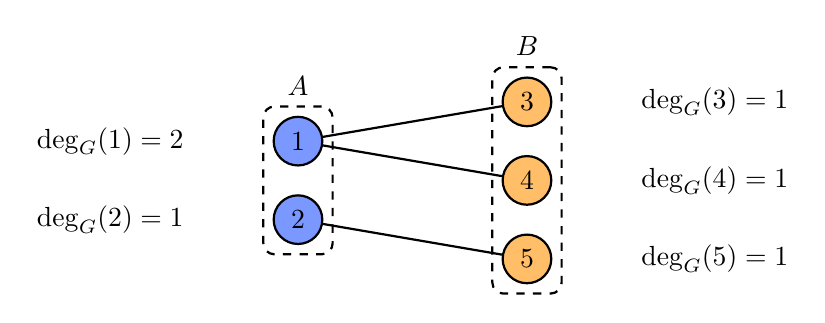
\begin{tikzpicture}[thick,amat/.style={matrix of nodes,nodes in empty cells,
  row sep=1em,draw,dashed,rounded corners,
  nodes={draw,solid,circle}},
  fsnode/.style={fill=myblue},
  ssnode/.style={fill=myorange}]

  \matrix[amat,nodes=fsnode,label=above:$A$] (mat1) {
  1\\
  2\\
  };

  \matrix[amat,right=2cm of mat1,nodes=ssnode,label=above:$B$] (mat2) {
  3\\
  4\\
  5\\};

  \node (1) [left = of mat1-1-1] {$\deg_G(1)=2$};
  \node (2) [left = of mat1-2-1] {$\deg_G(2)=1$};
  \node (3) [right = of mat2-1-1] {$\deg_G(3)=1$};
  \node (4) [right = of mat2-2-1] {$\deg_G(4)=1$};
  \node (5) [right = of mat2-3-1] {$\deg_G(5)=1$};
  \draw (mat1-1-1) edge (mat2-1-1);
  \draw (mat1-1-1) edge (mat2-2-1);
  %\draw (mat1-2-1) edge (mat2-2-1);
  \draw (mat1-2-1) edge (mat2-3-1);
\end{tikzpicture}
\caption{A simple bipartite graph.\label{fig:graph2}}
\end{figure}

If all vertices in a graph have the same degree, then the graph is called \emph{regular}.
For example, if every vertex in a bipartite graph has the same degree, then we call it regular bipartite graph.When each part of bipartite graph is regular, we call it \emph{biregular graph}.
In fact, we use notation $(d_A,d_B)$-biregular, where $d_A$ and $d_B$ denote the degrees of the nodes inside partitions $A$ and $B$ respectively.
We can see an example of a (3,2)-biregular in the figure \ref{fig:graph3}.
The bipartite graph in the figure \ref{fig:graph2} is not biregular because the nodes in part $A$ do not share degrees i.e. $\forall v, w \in A: \deg_G(v) = \deg_G(w)$ does not hold.

\begin{figure}[h]
\centering
% https://tex.stackexchange.com/a/499577
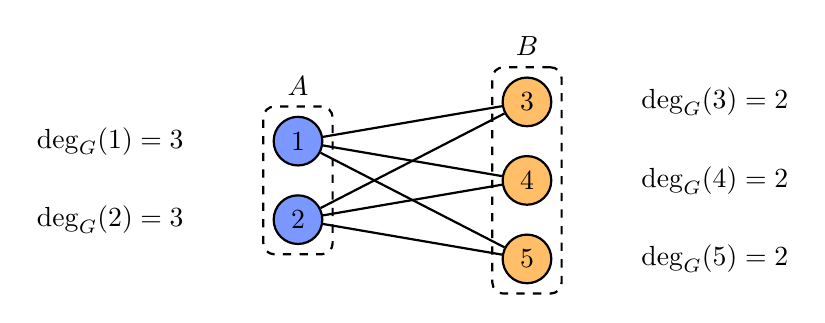
\begin{tikzpicture}[thick,amat/.style={matrix of nodes,nodes in empty cells,
  row sep=1em,draw,dashed,rounded corners,
  nodes={draw,solid,circle}},
  fsnode/.style={fill=myblue},
  ssnode/.style={fill=myorange}]

  \matrix[amat,nodes=fsnode,label=above:$A$] (mat1) {
  1\\
  2\\
  };

  \matrix[amat,right=2cm of mat1,nodes=ssnode,label=above:$B$] (mat2) {
  3\\
  4\\
  5\\};

  \node (1) [left = of mat1-1-1] {$\deg_G(1)=3$};
  \node (2) [left = of mat1-2-1] {$\deg_G(2)=3$};
  \node (3) [right = of mat2-1-1] {$\deg_G(3)=2$};
  \node (4) [right = of mat2-2-1] {$\deg_G(4)=2$};
  \node (5) [right = of mat2-3-1] {$\deg_G(5)=2$};
  \draw (mat1-1-1) edge (mat2-1-1);
  \draw (mat1-1-1) edge (mat2-2-1);
  \draw (mat1-1-1) edge (mat2-3-1);
  \draw (mat1-2-1) edge (mat2-1-1);
  \draw (mat1-2-1) edge (mat2-2-1);
  \draw (mat1-2-1) edge (mat2-3-1);
\end{tikzpicture}
\caption{A simple (3,2)-biregular graph.\label{fig:graph3}}
\end{figure}

A graph is considered as \emph{connected} if from every node one can traverse through the edges to all other nodes i.e. every pair of nodes need to also be connected.
For instance, the graph in figure \ref{fig:graph2} has two isolated vertex subsets $\{2, 5\}$ and $\{1, 3, 4\}$, therefore the graph is not connected.
On the other hand, the graphs on figures \ref{fig:graph1:b}, \ref{fig:graph1:c} and \ref{fig:graph3} are connected.
Let's not worry about the connectivity of the directed graph on figure \ref{fig:graph1:a} as directed graphs are not relevant to this work other than in this section.


\subsection{Distributed computing} \label{sec:distributed_computing}
Computing or processing a computer program in several identical or different computers is called distributed computing
\cite{DBLP:books/el/leeuwen90/LamportL90}.
It is similiar to running a computer program that contains multiple concurrent tasks, in a computer, but in distributed computing there are higher level tasks that are distributed to different computer nodes.

Computers are called nodes, and they are connected to each other with communication channels.
These communication channels carry data from node to another node.
Together, nodes and communication channels form a network.
A common way to visualize these networks is by drawing a graph in which the nodes represent computing nodes and edges represent the communication channels.
\cite{HirvonenSuomelaDistAlg2020}

\begin{figure}[h]
  \centering
  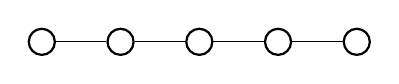
\begin{tikzpicture}[every node/.style={circle,thick,draw}]
  \node (1) {};
  \node (2) [ right of=1] {};
  \node (3) [ right of=2] {};
  \node (4) [ right of=3] {};
  \node (5) [ right of=4] {};
  \draw (1) -- (2);
  \draw (2) -- (3);
  \draw (3) -- (4);
  \draw (4) -- (5);
\end{tikzpicture}
\caption{Example of a small distributed network.}
\label{fig:dist_comp_1}
\end{figure}

According to Lamport \cite{DBLP:books/el/leeuwen90/LamportL90}, in the area of distributed computing, the term \emph{model} denotes a view or abstract representation of a distributed system.
There are multiple different computation models used in distributed computing.
The most important main category of distributed computation models is \emph{process models}.
In process models, the work or activities are represented as concurrently executed processes that execute their instructions sequentially.
The main way to distinguish different process models from each other is to categorise them by the method they use to communicate with each other (\emph{interprocess communication}).
\cite{DBLP:books/el/leeuwen90/LamportL90}


%\subsubsection{Message passing model} \label{sec:message_passing_model}
Message passing models are one form of a process model.
In the model, processes communicate by adding a message to a message queue, whether it is a shared or a process specific, and the recipient process moves the message out (dequeues) from the message queue.
\cite{DBLP:books/el/leeuwen90/LamportL90}

Different message passing models are widely used in the research field of distributed computing.
The models can varie in different details, such as in the size of the message queues \cite{DBLP:books/el/leeuwen90/LamportL90}, in the size of the messages \cite{peleg2000distributed} and on how the nodes get identified \cite{DBLP:conf/focs/Linial87}, if they are identified at all \cite{DBLP:conf/istcs/MayerNS95}.
%As the message passing models itself can be defined in multiple ways \cite{DBLP:books/el/leeuwen90/LamportL90}, we will use a definition from which the relevant models commonly inherit from.
We will dive deeper into the most relevant message passing models for this work in the following sections \ref{sec:port_number_model} and \ref{sec:local_model}.

An algorithm that is executed in a distributed fashion in a distributed network, is called as a distributed algorithm.
Each node in a network is started simultaneously and will always execute the same algorithm.
Initially the nodes are on the same state and there can be finitely or infinitely many states.
Initially the nodes are aware of only themselves and of the connections to their neighbours.
One might question that if every node starts with the same state, wouldn't they also end up in the same state?
Well yes, this happens inevitably in a case where the nodes were not given any additional symmetry breaking inputs and if every node sees the same amount of neighbours.
\cite{HirvonenSuomelaDistAlg2020}

%For example, we have a chain like network $W$ where each node $w$ has exactly two neighbours.
%The task is to execute an algorithm that finds the number of nodes in the network.


In practice, every computer node on a network has an UUID (Universally unique identifier) that can break the symmetry, and nodes are usually given some input data that they process, and nodes can always randomize data as they are never completely synchronized together, so this is not necessarily a problem.
In theory, we explicitly have to assume that there exists these kind of symmetry breaking elements.
In this works, distributed algorithms are deterministic unless otherwise mentioned.
In other research there might be randomizing involved.


\todo{Find a correct place to talk  about execution times if there is any}
In the message passing model, one could easily think that the execution time of the algorithm is the standard unit used to measure the performance but this is not true.
The message passing model implies that the dominant cost during an execution of a distributed algorithm is the message passing itself
\cite{DBLP:books/el/leeuwen90/LamportL90}.
This really... \todo{continue here}




%The following two sections (\ref{sec:port_number_model} and \ref{sec:local_model} ) talk about different forms of message passing models that are highly relative to this paper.

%In the theory of distributed computing, it is common to use terminology and concepts from graph theory as networks are basically graphs.
%With formal definitions, we can discuss more about the structure of distributed networks and reason features of those networks.
%We can further construct proofs of different theorems and so on. \todo{Fix this paragraph}

The algorithms that are executed in distributed fashion, are called distributed algorithms.
\todo{where to write about distributed algorithms?}
%A distributed algorithm is a specific type of algorithm that is executed in distributed fashion.
Specifically, each node executes the same algorithm.

%\todo{write about computation models, why they exist}


\subsubsection{Port number model} \label{sec:port_number_model}
This section is based on the course material from \cite{HirvonenSuomelaDistAlg2020} unless otherwise mentioned.

Port number model (PN model) is a rather weak model of computation that inherits from the message passing model.
In the model, nodes do not have identification.
An algorithm that executes in a port number model is called as a PN-algorithm.

We can basically take any network $N$ that has the same structure as a simple undirected graph $G$.
Each vertex of $G$ can be one-to-one mapped (bijection) to the nodes of $N$ and vice-versa.
Respectively all edges $\{v, w\}$ of $G$ can be mapped to communication channels between nodes $v$ and $w$.

Communication channels start and end from communication ports.
Each node has communication ports numbered from $1$ to $d$ where $d$ is the degree of the node.
The ports are numbered in an arbitrary order.

All nodes are considered identical, however nodes know their degree and it might differ between different nodes depending on the underlying graph $G$.
Every node starts the execution simultaneously following the same deterministic PN-algorithm $A$.
The execution of $A$ is done synchronously in parallel.
A communication round consists of following synchronous steps
\begin{enumerate}
  \item send message to each port,
  \item wait until all messages have been sent,
  \item receive a message from each port,
  \item update internal state.
\end{enumerate}
After each communication round, a node can optionally stop execution and announce its local output.
All nodes are required to eventually stop.
When all nodes have stopped, the algorithm is considered as stopped.
The running time of the algorithm $A$ is the total communication rounds that took place.








\subsubsection{Formalized port number model}
As in the previous section, this section is based on the course material from \cite{HirvonenSuomelaDistAlg2020} unless otherwise mentioned.

In the previous section \ref{sec:port_number_model} we introduced the PN model.
Now we give a formal definition of the PN model.

We call the network as a port number network or a PN-network
Port-numbering network is a 3-element tuple $N = (V, P, p)$, where $V$ and $P$ are the sets of vertices and ports respectively, and $p: P \rightarrow P$ is a function that maps a port to another port, forming a communication channel.
A port, an element of $P$, is a 2-element tuple $(v, i)$ where $v \in V$ and $i \in \{1, 2, ...\}$.
Additionally we assume that $p$ is an involution, that is, $\forall x \in P : p(p(x)) = x, $ i.e. each edge of the underlying graph is undirected.
See the figures \ref{fig:formal_pn1:a} and \ref{fig:formal_pn1:b} for examples of valid and invalid PN networks.

\begin{figure}[h]
  \subcaptionbox{A PN network of two nodes, $a$ and $b$.
    Both $a$ and $b$ have degree of 2, therefore 2 ports.
    Ports are $(a, 1), (a, 2), (b, 1)$ and $(b, 2)$.
    The connections are
      $p((a, 1)) = (b, 1)$,
      $p((a, 2)) = (b, 2)$,
      $p((b, 1)) = (a, 1)$ and
      $p((b, 2)) = (a, 2)$.
    \label{fig:formal_pn1:a}
  }%
    [.45\linewidth] {
    \centering
    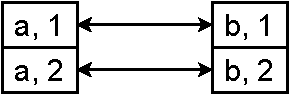
\includegraphics[scale=0.6]{diagrams/formalizing_pn_network_diagram1.pdf}
  }
  \hfill
  \subcaptionbox{
    An invalid PN network as port mapping function $p$ is not an involution:
    $p(p((a, 1))) = p(p((a, 2))) \neq (a, 1)$.
    \label{fig:formal_pn1:b}
  }%
    [.45\linewidth] {
    \centering
    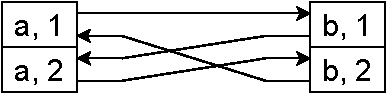
\includegraphics[scale=0.6]{diagrams/formalizing_pn_network_diagram2.pdf}
  }
  \caption{Examples of a valid and an invalid PN network.}
  \label{fig:formal_pn1}
\end{figure}


The degree $\deg_N(v)$ of a node $v \in V$ is equal to the number of ports of $v$.
We assume that the port numbers are consecutive positive integers starting from 1, i.e. the ports of a node $v$ are $\{(v, i) | i \in \{1, 2, ..., \deg_N(v)\}\}$.
Note that the highest port number of $v$ is also the degree of $v$.

When we say \emph{port number $i$ in node $v$}, we refer to the port $(v, i)$.
When we say \emph{port $(v, i)$ is connected to port $(w, j)$}, we refer to $p((v, i)) = (w, j)$.

A loop is a connection where port $(v, i)$ is connected to port $(v, j)$.
For example there are two loops, p((a, 1)) = p((a, 2) and p((c,2)) = (c,2), in the figure \ref{fig:formal_pn2:c}.

There are multiple connections between two distinct nodes $v$ and $w$, if $p((v, i_1)) = (w, j_1)$, $p((v, i_2)) = (w, j_2)$, $i_1 \neq j_1$ and $i_2 \neq j_2$.
For example the connections $p((b, 2)) = (d, 1)$ and $p((b, 3)) = (d, 2)$ in the figure \ref{fig:formal_pn2:c}.

If a PN network has neither loops or multiple connections, it is called a \emph{simple} network.
For example the network is simple in the figure \ref{fig:formal_pn2:a}.

Each simple PN network $N=(V,P,p)$ also has a thing called an underlying graph $G=(V,E)$.
An edge $(v, w)$ is part of the underlying network if and only if $v$ and $w$ are connected, that is, $E = \{ \{v, w\} \, | \,  p((v, i)) = (w, j) \}$ where ${v, w} \in E$.

\begin{figure}[h]
  \subcaptionbox{
    A simple PN network.
    The underlying graph is also simple.
    \label{fig:formal_pn2:a}
  }%
    [.3\linewidth] {
    \centering
    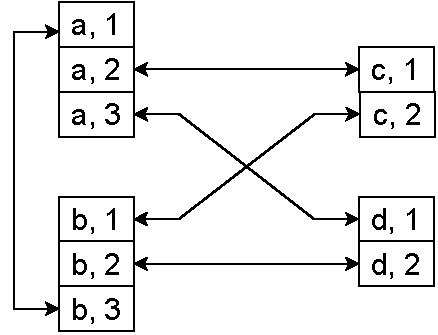
\includegraphics[scale=0.6]{diagrams/formalizing_pn_network_diagram4.pdf}
  }
  \hfill
  \subcaptionbox{
    An alternative representation of the PN network from figure \ref{fig:formal_pn2:b}
    \label{fig:formal_pn2:b}
  }%
    [.3\linewidth] {
    \centering
    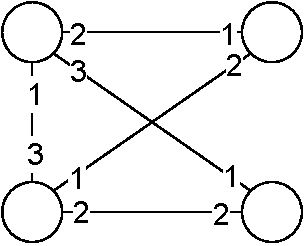
\includegraphics[width=0.3\textwidth]{diagrams/formalizing_pn_network_diagram5.pdf}
  }
  \hfill
  \subcaptionbox{
    A PN network with loops and parallel connections.
    This kind of network cannot be shown in the alternative representation unlike the network on figure \ref{fig:formal_pn2:a}.
    \label{fig:formal_pn2:c}
  }%
    [.3\linewidth] {
    \centering
    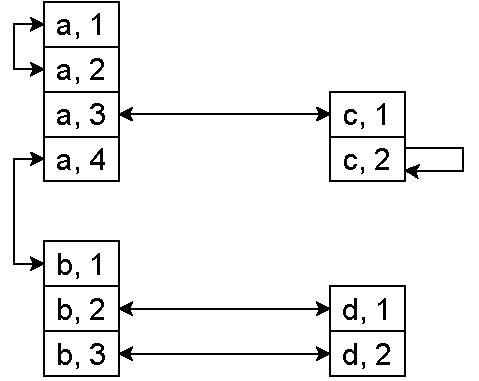
\includegraphics[scale=0.6]{diagrams/formalizing_pn_network_diagram3.pdf}
  }
  \caption{Examples of simple and non simple PN networks.}
  \label{fig:formal_pn2}
\end{figure}


%\todo{continue from here on  TUESDAY 4.1.2022}



\todo{Add formal definition of the PN algorithm}
Port numbering algorithm is ...



\subsubsection{LOCAL model} \label{sec:local_model}

\subsection{LCL problems} \label{sec:lcl_problems}

\subsection{Boolean satisfiability problem}

\subsection{Previous research} \label{sec:previous_research}

\todo{Especially LCL classification research}

\clearpage



\clearpage
%!tex root = ../main.tex
%% Research
%%
%% Instructions in Finnish:
%% Tässä osassa kuvataan käytetty tutkimusaineisto ja tutkimuksen metodologiset
%% valinnat, sekä kerrotaan tutkimuksen toteutustapa ja käytetyt menetelmät.
\section{Research material and methods}

\todo{Under the methods, I can write about software development methods used. Remember that }
\todo{LCL problems from LCL classifier's database are probably research material}



\clearpage
%!tex root = ../main.tex
%% Implementation
%%


%\section{Automatically proving lower bounds for LCL problems} \label{sec:implementation}
\section{Implementation} \label{sec:implementation}
In this chapter we will cover all the important topics that are used in the actual implementation.
The implementation itself is a tool, that attempts to automatically find a proof that shows the given LCL problem to be impossible to be solved in PN model (see section \ref{sec:port_number_model} for more information about PN model).
\todo{should the discussion of the implementation be after explanation of the topics?}

\subsection{The idea}
Given an LCL problem, the goal is to find a proof that it is impossible to solve the problem in PN model.
To prove this, we first assume the oppisite, that it is possible to solve the problem in PN model.
Then we try to find a counterexample that shows the assumption to be false, therefore it is impossible to solve the problem in PN model.
A graph in which we cannot find any viable labelling is a good counterexample, as this directly shows that we cannot solve the LCL problem in every graph, therefore it is impossible to solve in PN model.

For each pair of LCL problem and graph, we want to be able to check if labelling is impossible.
To perform the checking, we first encode the problem and graph into a SAT problem.
Then we leverage the power of SAT solvers to solve the SAT problem.
We feed the SAT problem into the solver, which returns either SAT (satisfiable) or UNSAT (unsatisfiable) as a result.
In case the result is UNSAT, we have found a counterexample and we are done.
Otherwise we can continue searching using some other graph.

We can repeat this routine for each graph in the current search space.
Deciding the search space is up to the end user.
A search space can be for example every graph from $n=1$ to $n=10$.
$|V| \in \{1, 2, ..., n\}$
A good strategy is to first start with small graphs and increase the size of graphs as smaller if needed.
A search space could be for example every graph 


\begin{figure}[h]
\centering
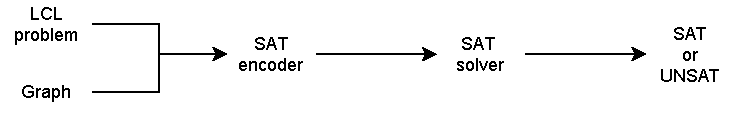
\includegraphics[]{diagrams/implementation_idea_diagram.pdf}
\caption{The process of finding negative results when given a graph and an LCL problem.}
\label{fig:implementatio:idea:1}
\end{figure}
%This is indeed what we have used in this work.
%Probably, we have to iterate a lot of graphs.
%For this purpose we want to be able to generate the graphs.




\subsection{Generating LCL-problems}
\todo{parallelization}
\subsection{Generating graphs}
\todo{parallelization}
\subsection{SAT encoding and solving}
\todo{parallelization?}
%\subsection{Software optimizations}
\subsection{Caching}
\todo{pre-computing multigraphs}
\todo{pre-computing lcl problems (and power sets of lcl problems)}
\todo{caching}

\subsection{parallelization}
\todo{Talk about parallelization here or separately in above sections}



\clearpage
%!tex root = ../main.tex
%% Results
%%

\section{Results} \label{sec:results}
\todo{Show all results that have been found while doing the research, like different problems that have now new lower bounds.}



\clearpage
%!tex root = ../main.tex
%% Summary
%%

\section{Summary} \label{sec:summary}



\clearpage
\thesisbibliography
\printbibliography


\clearpage

\thesisappendix

\section{First example appendix\label{AppendixA}}

\clearpage
\section{Second example appendix\label{AppendixB}}


\end{document}
